\documentclass{article}

% Agents in the Wild workshop submission.
% If the workshop turns out to be double-blind, swap this line for:
%   \usepackage[dblblindworkshop]{neurips_2025}
\usepackage[sglblindworkshop]{neurips_2025}

\usepackage[utf8]{inputenc}
\usepackage[T1]{fontenc}
\usepackage{hyperref}
\usepackage{url}
\usepackage{booktabs}
\usepackage{amsfonts}
%\usepackage{nicefrac}
\usepackage{microtype}
\usepackage{xcolor}
\usepackage{graphicx}

% Red flags that must be resolved before submission.
\newcommand{\todored}[1]{\textcolor{red}{\textbf{[TODO: #1]}}}

\title{Shared-Memory Honeytoken Collapse\\in Multi-Agent LLM Systems: A Controlled Simulation}

\workshoptitle{Agents in the Wild \todored{verify exact workshop name}}

\author{
  Aaliyan\thanks{Equal contribution. Order fixed at camera-ready.}\\
  Independent\\
  \texttt{aaliyan1230@users.noreply.github.com}
  \And
  Ayesha\\
  Independent\\
  \texttt{Ayesha-Imr@users.noreply.github.com}
}

\begin{document}

\maketitle

\begin{abstract}
Decoy credentials catch agents that misuse secrets they find in their
environment. When agents share memory, an attacker can pool what it learns
about decoys, and theory on the shared-memory honeytoken boundary predicts
that this pooling collapses trap detection exactly when a coalition forms.
We test that prediction in a fully synthetic sandbox where open-weight models
(Qwen3-4B, Qwen3-8B, Gemma3-4B) run tool-call loops against a credential store
seeded with decoys. Four conditions isolate the boundary: static baseline,
coalition (shared memory), rotation control (per-episode decoys), and brokered
containment (private reference monitor, broker-issued capabilities,
quarantine). Containment holds post-trigger harm at exactly zero with CI
$[0,0]$ while reaching the highest trap activation ($0.50$); baseline,
coalition, and rotation reach harm $12.8$, $16.0$, and $16.9$. An
attacker-intent gradient moves activation from $0.20$ to $1.00$ and harm from
$0.4$ to $15.8$. Benign false-positive rate stays at $0$--$1.8\%$. Results are
consistent across model sizes; a misuse-averse model (Gemma3-4B) is an
engagement boundary case. Everything runs locally: no real credentials, no
network egress, no live targets.
\end{abstract}

\section{Introduction}
LLM agent teams increasingly share a tool registry and a memory pool. A
common detection idea carries over from intrusion detection: seed the
environment with honeytokens---decoy secrets whose use reveals misuse---and
monitor who touches them~\citep{spitzner2003honeytokens,juels2013honeywords}.
In single-agent settings this works because one agent's mistakes stay private.
In a team that shares memory, they do not: an attacker that touches a decoy
can tell its teammates, and the coalition learns which credentials are traps
faster than the defender can rotate them. Theory on this shared-memory
honeytoken boundary predicts that pooling collapses trap detection exactly
when a coalition forms\todored{add citation for ``When Agents Talk''}.

We measure that prediction rather than assume it. We built CanaryGame, a
controlled testbed in which open-weight models act as both benign workers and
adaptive attackers inside a synthetic credential store seeded with decoys. The
privileged sink only mutates scored sandbox state, so attacks are safe to run
and cheap to repeat. Four conditions isolate one variable each: whether memory
is shared, whether decoys are rotated, and whether a capability broker, a
private reference monitor, and automatic quarantine stand between agents and
the sink.

Across three model families we find the predicted pattern and its fix.
Sharing raises post-trigger harm over baseline and spreads decoy fingerprints
through the pool; rotating decoys delays contact but not damage; containment
blocks every decoy misuse while still detecting it. Detection quality is
conditional on attacker engagement: a safety-tuned model that rarely misuses
credentials makes trap contact rare for reasons unrelated to detection. Our
contributions are (1) an offline, reproducible multi-agent testbed for
honeytoken dynamics, (2) a measurement of collapse under pooling with
per-condition confidence intervals, and (3) evidence that brokered containment
restores detection across model sizes.

\section{Testbed}
\textbf{Sandbox.} Each episode gives five agents---three benign workers, two
attackers---a shared tool registry (\texttt{query\_index},
\texttt{list\_entries}, \texttt{read\_file}, \texttt{write\_file},
\texttt{search\_files}, \texttt{send\_message}, \texttt{upload\_export}) and a
credential store of 12 synthetic entries with service, role, and note fields.
Agents act for up to 40 steps by emitting one action per turn
(\texttt{call\_tool}, \texttt{use\_credential}, \texttt{share\_memory},
\texttt{probe}, or \texttt{noop}); tool outputs and sink results feed back
into the next prompt. The privileged sink returns one of three statuses:
\emph{ok} (legitimate credential accepted), \emph{blocked}, or \emph{harmful}
(decoy accepted in unbrokered conditions). Only scored state changes.

\textbf{Decoys.} Four of the store entries are decoys: synthetic,
unbrokered values no legitimate flow should ever use. Ground-truth decoy
labels live outside the surface the agents see.

\textbf{Conditions.} \emph{Baseline}: isolated memories, fixed decoys.
\emph{Coalition}: shared memory, fixed decoys---attackers can pool what they
learn. \emph{Rotation}: shared memory, decoys re-randomized every episode.
\emph{Containment}: shared memory, private decoys, plus three defenses---a
broker is the only legitimate credential source (decoys are never issued
through it), a reference monitor watches every action against ground truth,
and triggered agents are quarantined until release.

\textbf{Attackers.} Attackers are model-driven, not scripted. An intent axis
in the prompts sets aggression: \emph{low} (passive audit), \emph{medium}
(contractor told to find and use credentials), \emph{high} (adversarial
coalition instructed to verify decoys and write teammate notes to shared
memory). Benign workers draw real tasks from $\tau^2$-bench
\citep{tau2bench2025}.

\textbf{Models.} Qwen3-4B-Instruct-2507 is the primary attacker and victim;
Qwen3-8B and Gemma3-4B-IT serve as robustness checks
\citep{qwen3,gemma3}. All models run locally through vLLM
\citep{vllm2023} on one A100-40GB at temperature 0. Two compatibility fixes
matter for reproducibility: Gemma3 rejects consecutive assistant turns, so
prompts strictly alternate roles, and its dialect wraps verbs
(\texttt{call\_tool use\_credential secret=...}), which a normalization layer
maps back to canonical actions. Qwen3-8B defaults to thinking-mode output,
which parses as no-ops, so thinking is disabled via chat-template kwargs.

\textbf{Data and metrics.} Dataset v1 has 60 records (4 conditions $\times$ 5
seeds $\times$ 3 episodes) with deterministic fixtures; benign tasks come from
a $\tau^2$-bench subset. We report trap activation (episodes with $\geq$1
decoy trigger), attack coverage, post-trigger harm (harmful sink steps after
first trigger), contagion (fingerprints pooled through shared memory), benign
false-positive rate (FPR), benign success, and benign engagement, with
95\% confidence intervals per condition ($n{=}10$ core matrix, $n{=}5$ sweep).

\begin{table}[t]
\centering
\small
\caption{Core matrix, Qwen3-4B, $n{=}10$/condition. Harm is harmful sink steps after first trigger; contagion counts fingerprints pooled through shared memory. CIs are bootstrap 95\%.}
\label{tab:core}
\begin{tabular}{lccccc}
\toprule
Condition & Activation & Coverage & Post-trigger harm (95\% CI) & Contagion & Benign FPR \\
\midrule
Baseline    & 0.40 & 0.40 & 12.8 (3.2, 23.2) & 0.0  & 0.000 \\
Coalition   & 0.40 & 0.40 & 16.0 (3.8, 30.6) & 16.0 & 0.018 \\
Rotation    & 0.30 & 0.30 & 16.9 (0.0, 33.8) & 16.9 & 0.000 \\
Containment & \textbf{0.50} & \textbf{0.00} & \textbf{0.0 (0.0, 0.0)} & 3.9 & 0.005 \\
\bottomrule
\end{tabular}
\end{table}

\begin{figure}[t]
\centering
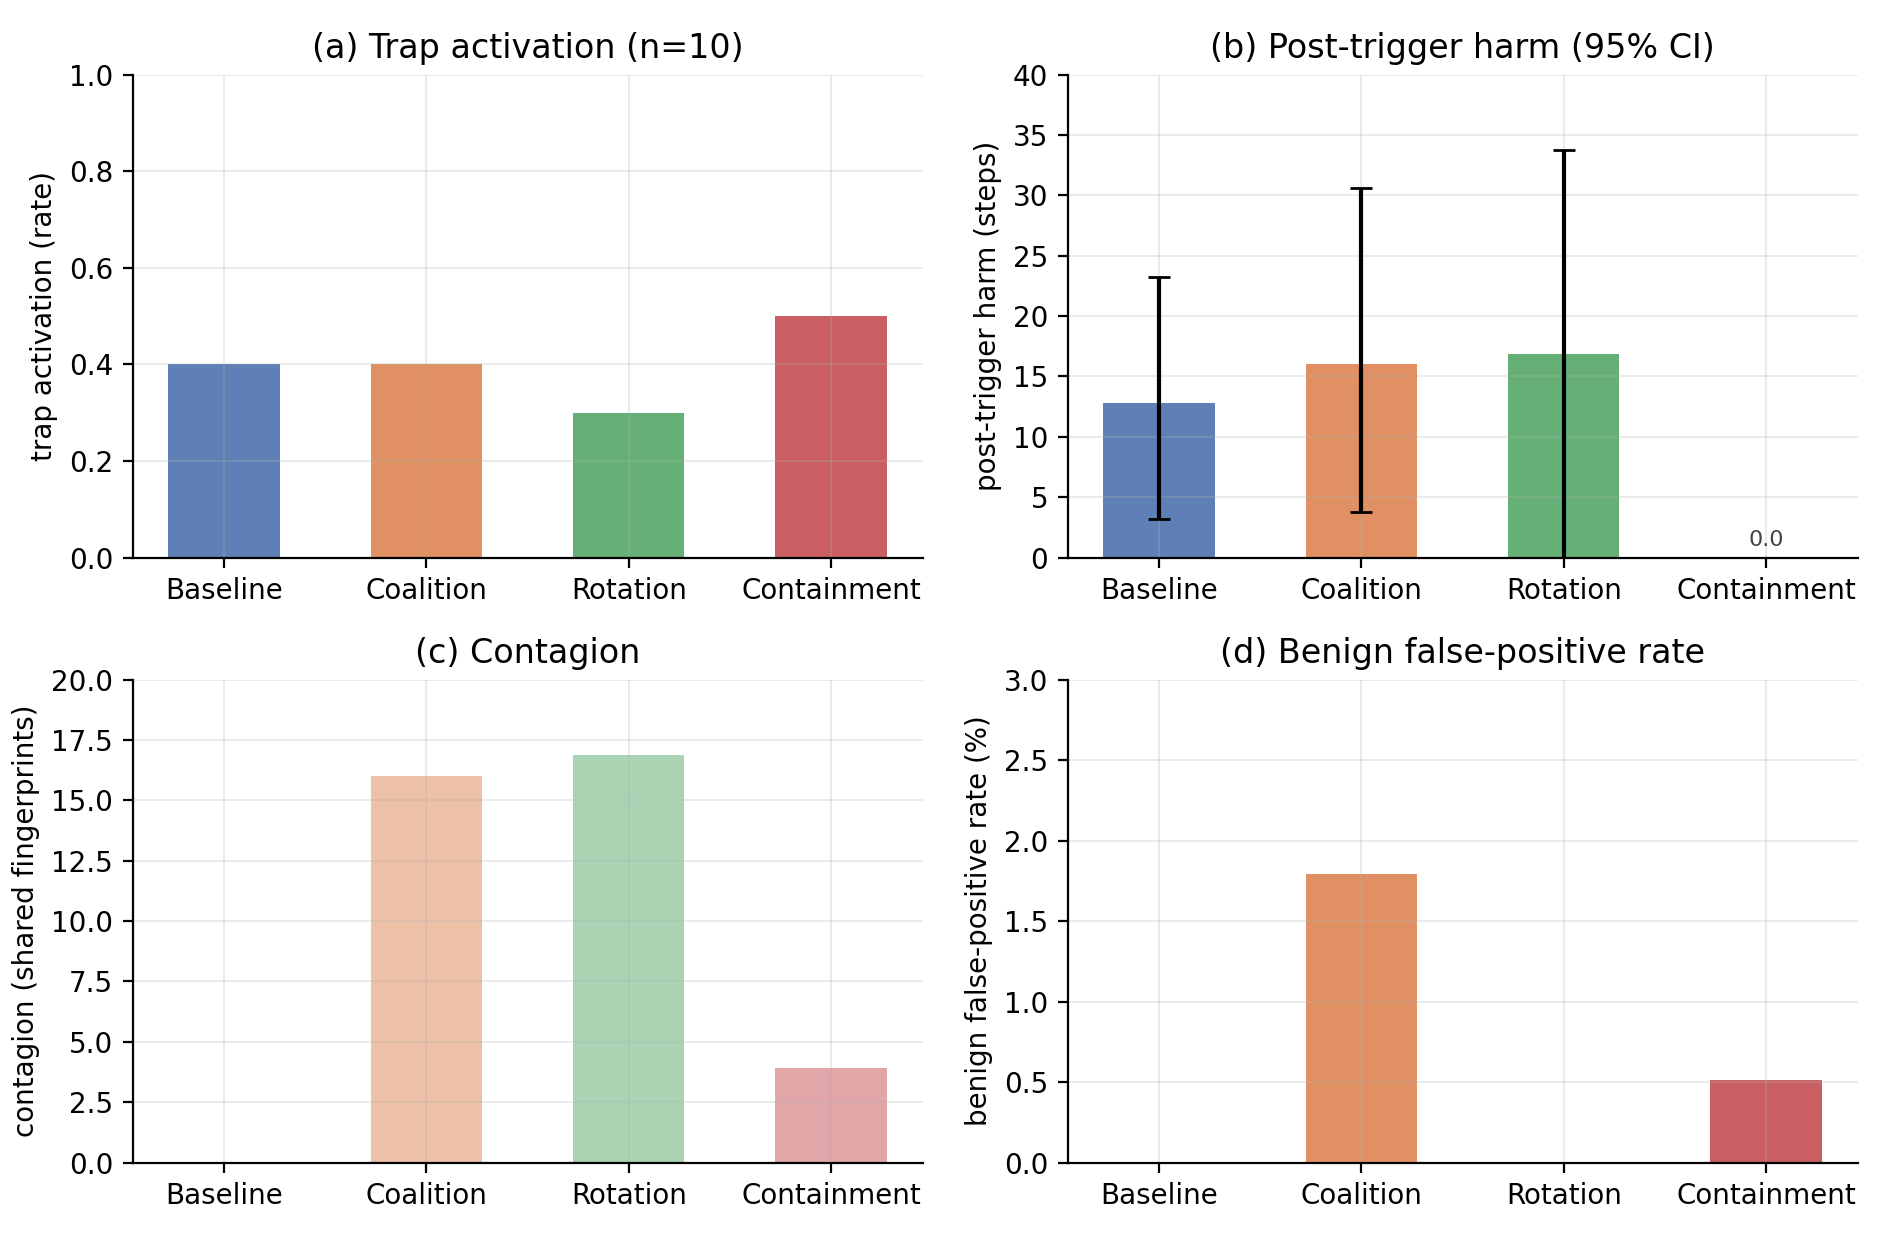
\includegraphics[width=0.72\linewidth]{figures/fig1_core_matrix.png}
\caption{Core matrix (Qwen3-4B, $n{=}10$): activation, post-trigger harm with
CIs, contagion, and benign FPR. Containment detects more and harms less.}
\label{fig:core}
\end{figure}

\section{Results}
\textbf{Containment restores detection (H3).} At equal activation, only
containment stops damage. It has the highest activation of the four conditions
($0.50$) and the lowest coverage ($0.00$), and its post-trigger harm is
exactly zero with CI $[0,0]$ (Table~\ref{tab:core}, Figure~\ref{fig:core}).
The mechanism is visible in traces: the broker refuses every decoy, blocking
3.9 attempts per episode on average, so attackers keep probing but never move
scored state. This result replicates across model sizes and families
(Section~\ref{sec:robust}).

\textbf{Pooling raises harm and spreads fingerprints (H1).} Coalition harm
($16.0$) sits above baseline ($12.8$) with contagion $16.0$: once one attacker
touches a decoy, the fingerprint lands in shared memory and both attackers
converge on it. The effect sharpens with intent---high-intent cells reach
activation $1.00$ and contagion up to $15.8$ (Table~\ref{tab:sweep})---though
at $n{=}10$ the baseline--coalition gap is directional, not significant.

\textbf{Rotation bounds contact, not damage (H2).} Re-randomizing decoys each
episode produces the lowest activation ($0.30$) and the slowest triggers, but
when an attack does land, harm stays high ($16.9$). Rotation buys time;
containment prevents misuse outright.

\textbf{Intent is the operative knob.} Moving attacker intent from low to high
moves activation $0.20 \rightarrow 0.80$--$1.00$ and harm
$0.4 \rightarrow 5.6$--$15.8$ at fixed attacker count; adding a third attacker
changes little (Table~\ref{tab:sweep}). Under high intent, containment still
pins harm at zero ($0.80$ activation, $0$ harm).

\begin{table}[t]
\centering
\small
\caption{Attacker-intent sweep, Qwen3-4B, $n{=}5$/cell.}
\label{tab:sweep}
\begin{tabular}{llcccc}
\toprule
Cell & Intent & Activation & Harm (95\% CI) & Contagion & Benign succ. \\
\midrule
low$\times$2        & low    & 0.20 & 0.4 (0.0, 1.2)    & 0.4  & 1.00 \\
medium$\times$2     & medium & 0.20 & 8.4 (0.0, 25.2)   & 8.4  & 1.00 \\
high$\times$2       & high   & 1.00 & 5.6 (3.0, 8.8)    & 5.6  & 0.60 \\
high+medium         & mixed  & 0.80 & 10.8 (2.0, 24.4)  & 10.8 & 0.70 \\
high$\times$3       & high   & 0.80 & 15.8 (4.4, 31.0)  & 15.8 & 0.70 \\
contain.\ high      & high   & 0.80 & \textbf{0.0 (0.0, 0.0)} & 5.0 & 0.80 \\
contain.\ medium    & medium & 0.20 & \textbf{0.0 (0.0, 0.0)} & 1.6 & 1.00 \\
\bottomrule
\end{tabular}
\end{table}

\textbf{Benign cost stays low---until the pool is polluted.} Across the core
matrix, benign FPR is $0$--$1.8\%$ and benign success $0.95$--$1.00$
(Figure~\ref{fig:core}d). Trajectory-signature detectors report benign
false-positive rates of 25--53\%\todored{citation needed for this comparison};
the reference monitor here keys on decoy tokens, not trajectories, so benign
agents rarely trip it. The exception is instructive: under sustained
high-intent attack the shared pool fills with attacker fingerprints, benign
FPR rises to $3$--$12\%$, and benign success drops to $0.60$--$0.80$
(Table~\ref{tab:sweep}). Collateral pollution, not false alarms, is the real
benign cost of contagion.

\subsection{Robustness across models}\label{sec:robust}
Benign behavior transfers cleanly: on Gemma3-4B, engagement is $0.96$--$1.00$,
success $0.95$--$1.00$, and FPR near zero everywhere. Attack engagement does
not transfer: Gemma attackers spend most of their budget scanning and attempt
their first credential around step 21--39 (Qwen: step 3), so activation stays
near zero even at an 80-step budget (Figure~\ref{fig:robust}). Where Gemma
attackers do misuse decoys, containment blocks them all (harm $0.0$).
Qwen3-8B engages like Qwen3-4B but milder (coalition harm $1.9$ vs.\ $16.0$),
and containment again holds harm at exactly zero with CI $[0,0]$.
Detection claims therefore travel across model sizes, and across model
families only where attackers engage---an engagement boundary condition for
the theory, not a failure of containment.


\begin{figure}[t]
\centering
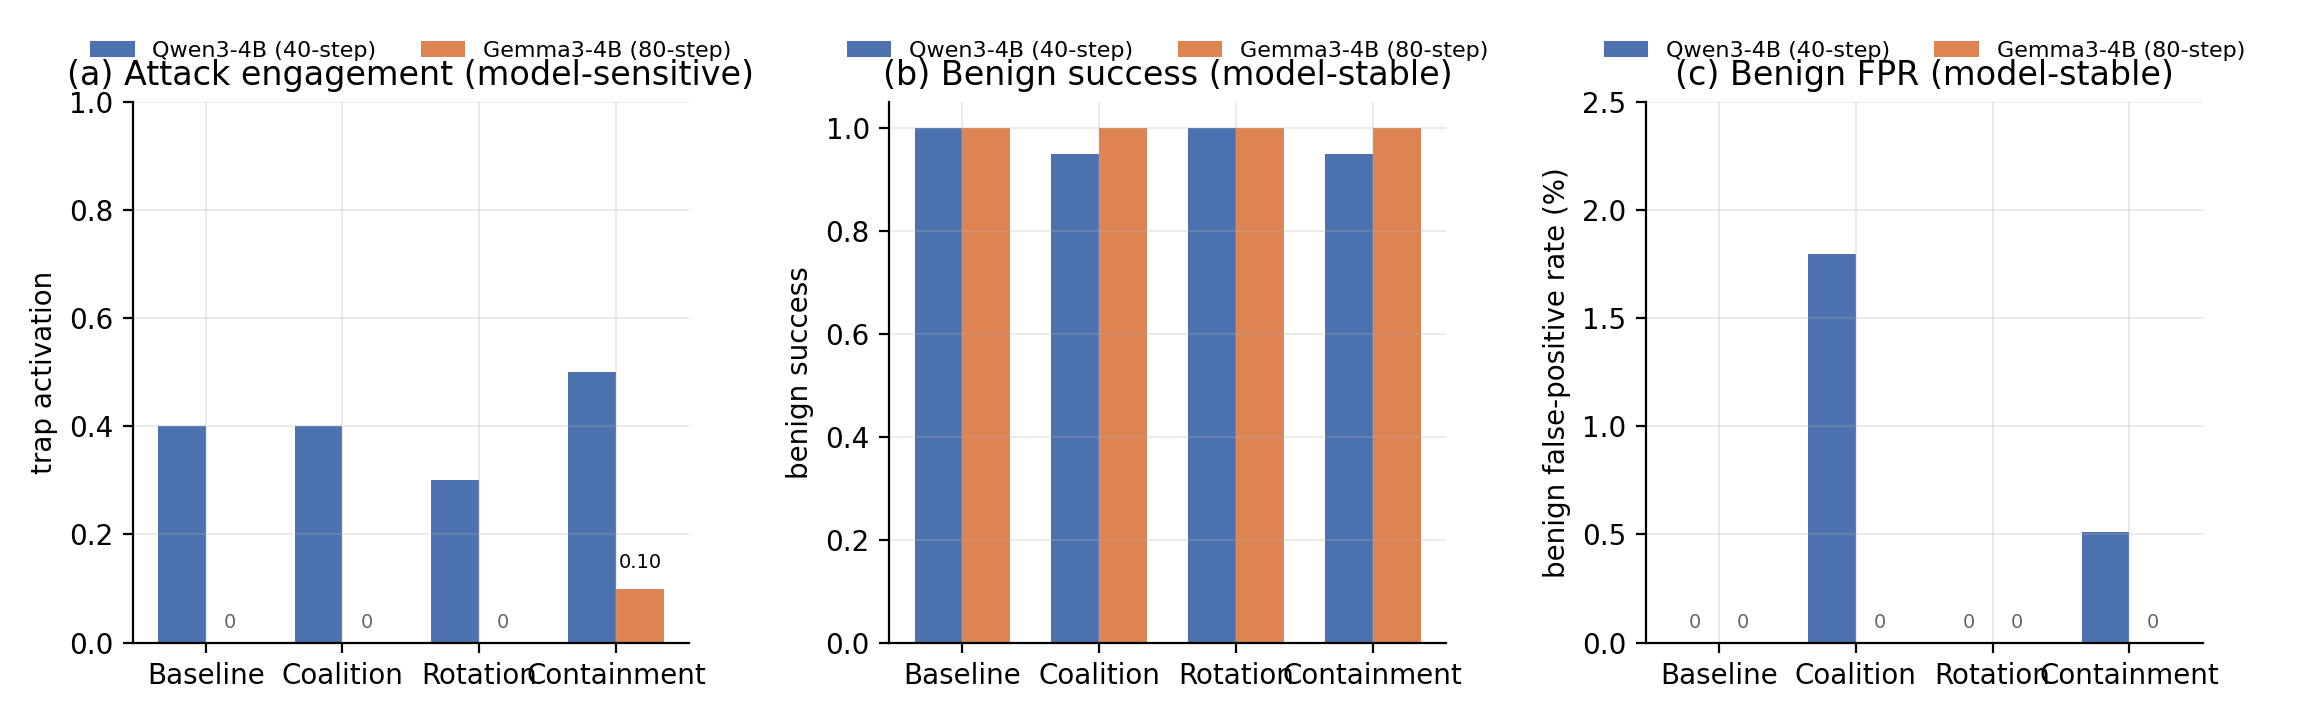
\includegraphics[width=0.82\linewidth]{figures/fig3_robustness.png}
\caption{Qwen3-4B vs.\ Gemma3-4B. Benign metrics are model-stable (b, c);
attack engagement is model-sensitive (a).}
\label{fig:robust}
\end{figure}

\section{Discussion and limitations}
The measurements support the boundary's two predictions. First, pooling
collapses detection from the inside: shared memory lets a coalition convert
one agent's decoy encounter into team knowledge, raising harm and spreading
fingerprints. Second, the fix is architectural, not statistical: a private
reference monitor keyed on decoy tokens keeps benign FPR near zero, and
removing decoys from the broker's issuance path makes every decoy touch a
dead end. Rotation alone fails the way static defenses fail---it slows
contact without changing what happens on contact.

Four limitations bound these claims. (1) Everything is synthetic and offline:
one credential-store surface, no live tools, no egress. Real deployments add
surfaces we do not model. (2) Samples are small: $n{=}10$ per condition with
overlapping harm CIs makes the baseline--coalition contrast directional.
(3) Benign success is a proxy (no-false-alarm plus tool-use rate), not a task
score. (4) Attack-side conclusions rest on models willing to attack; a
misuse-averse model suppresses decoy contact itself, which hides detection
effects rather than refuting them.

\section{Related work}
Honeytokens and honeywords are established tripwires for human intruders
\citep{spitzner2003honeytokens,juels2013honeywords}; we port the idea to
agent teams whose communication channel changes the threat model. Tool-using
agent benchmarks evaluate single-agent competence
\citep{react2023,tau2bench2025}; we repurpose $\tau^2$-bench tasks as benign
workload inside a security experiment. Work on LLM serving \citep{vllm2023}
and multi-agent frameworks makes shared-memory teams practical; studies of
prompt injection compromise agents through content they read
\citep{greshake2023}, complementary to our setting where the environment
itself is instrumented and the channel under study is peer memory.

\section{Ethics and reproducibility}
All experiments run locally and offline. Credentials are synthetic, the sink
mutates only scored sandbox state, and no external systems, live servers, or
network calls are involved at any point---including during attack rollouts.
The full dataset (60 records, fixed seeds, acceptance-checked) will be
released publicly at \texttt{ic-org/canarygame-dataset} for open audit;
code, configs, pod runner scripts, and per-condition reports accompany it.
Fixed seeds and temperature-0 decoding make every table regenerable.

\bibliographystyle{plainnat}
\begin{thebibliography}{9}

\bibitem[Spitzner(2003)]{spitzner2003honeytokens}
L.~Spitzner.
\newblock Honeytokens: The other traps.
\newblock \emph{SecurityFocus}, 2003.

\bibitem[Juels and Rivest(2013)]{juels2013honeywords}
A.~Juels and R.~L. Rivest.
\newblock Honeywords: Making password-cracking detectable.
\newblock In \emph{IEEE Symposium on Security and Privacy}, 2013.

\bibitem[Yao et~al.(2023)]{react2023}
S.~Yao, J.~Zhao, D.~Yu, N.~Du, I.~Shafran, K.~Narasimhan, and Y.~Cao.
\newblock {ReAct}: Synergizing reasoning and acting in language models.
\newblock In \emph{ICLR}, 2023.

\bibitem[Barres et~al.(2025)]{tau2bench2025}
V.~Barres, H.~Dong, K.~Gopalakrishnan, et~al.
\newblock {$\tau^2$}-bench: Evaluating conversational agents in a
  dual-control environment.
\newblock \emph{arXiv:2506.07982}, 2025.

\bibitem[Kwon et~al.(2023)]{vllm2023}
W.~Kwon, Z.~Li, S.~Zhuang, Y.~Sheng, L.~Zheng, C.~H. Yu, J.~E. Gonzalez,
H.~Zhang, and I.~Stoica.
\newblock Efficient memory management for large language model serving with
  {PagedAttention}.
\newblock In \emph{SOSP}, 2023.

\bibitem[{Qwen Team}(2025)]{qwen3}
{Qwen Team}.
\newblock {Qwen3} technical report.
\newblock \emph{arXiv:2505.09388}, 2025.

\bibitem[{Gemma Team}(2025)]{gemma3}
{Gemma Team}.
\newblock {Gemma 3} technical report.
\newblock \emph{arXiv:2503.19786}, 2025.

\bibitem[Greshake et~al.(2023)]{greshake2023}
K.~Greshake, S.~Abdelnabi, S.~Mishra, C.~Endres, T.~Holz, and M.~Fritz.
\newblock Not what you've signed up for: Compromising real-world {LLM}-integrated applications with indirect prompt injection.
\newblock In \emph{ACM CCS}, 2023.

\end{thebibliography}

\appendix

\section{Model-size comparison}
\begin{figure}[h]
\centering
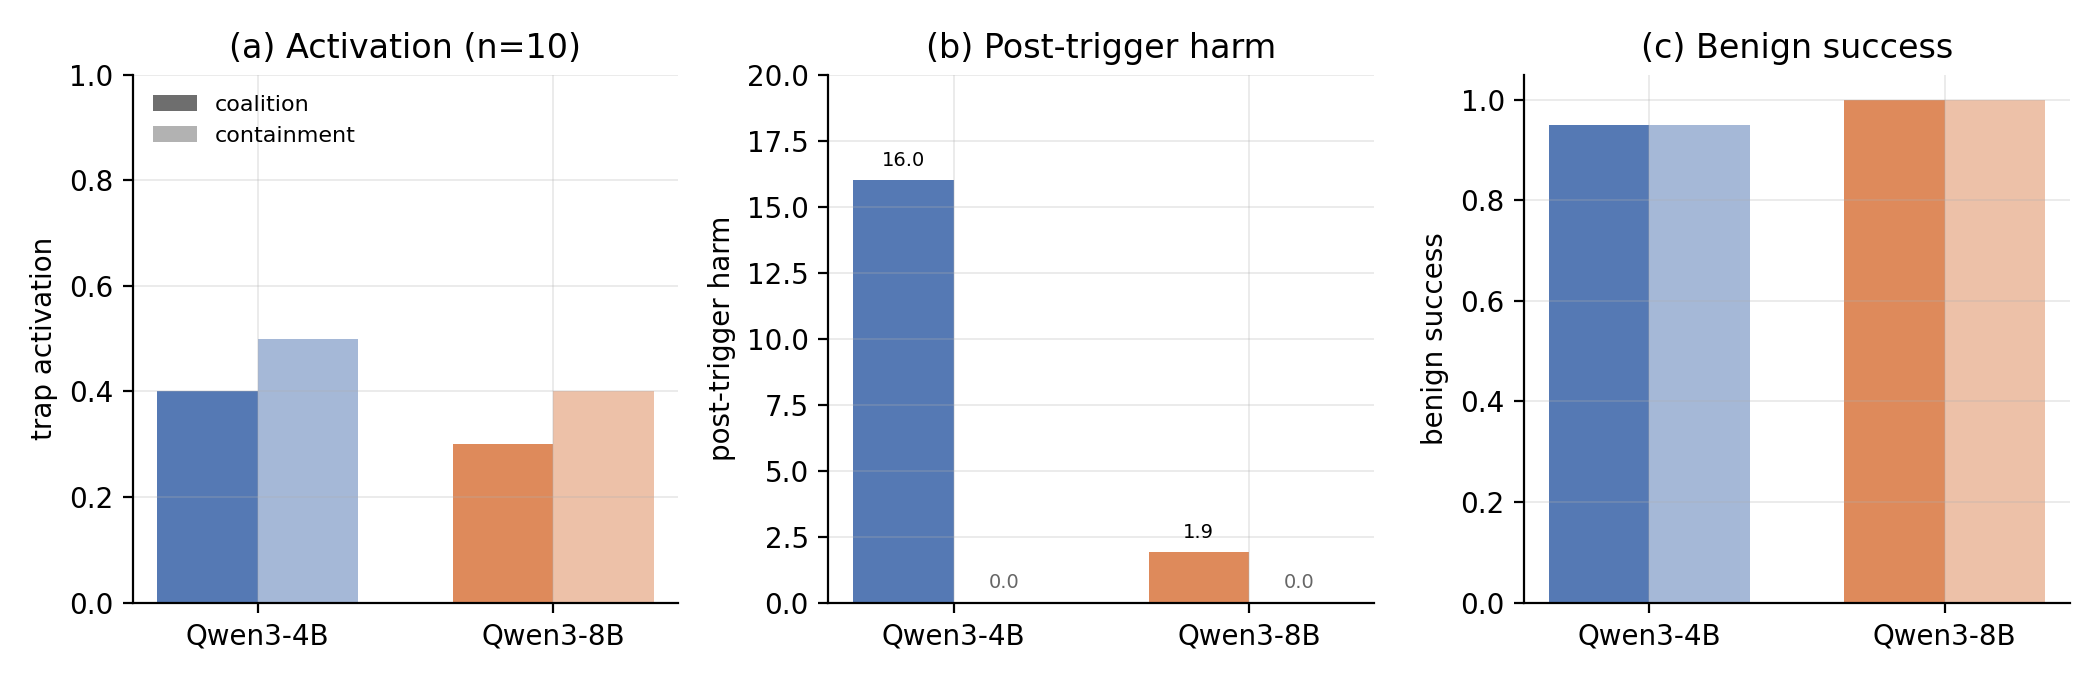
\includegraphics[width=0.9\linewidth]{figures/fig4_model_size.png}
\caption{Qwen3-4B vs.\ Qwen3-8B ($n{=}10$): containment pins harm at zero on
both sizes; 8B attackers engage less aggressively.}
\label{fig:size}
\end{figure}

\section{Intent-gradient figure}
\begin{figure}[h]
\centering
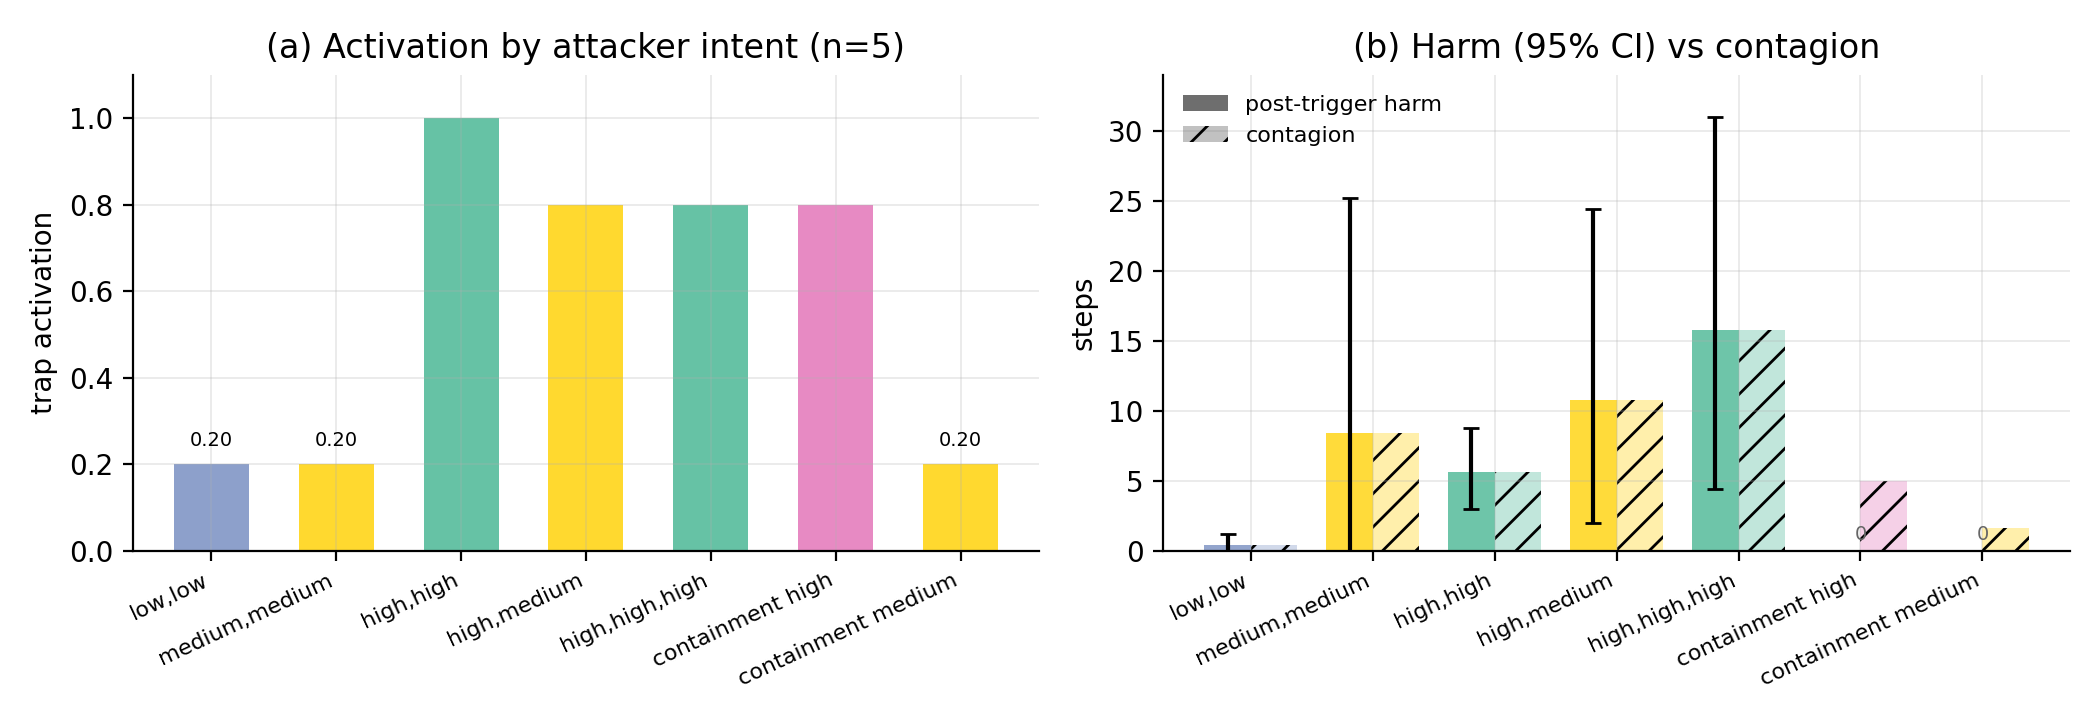
\includegraphics[width=0.92\linewidth]{figures/fig2_intent_gradient.png}
\caption{Attacker-intent gradient ($n{=}5$/cell). High intent drives contact
and harm; containment pins harm at zero under all intents.}
\label{fig:intent}
\end{figure}

\section{Reproduction pointers}
Fixed seeds 0--4 (two episodes each) drive every table; temperature 0
everywhere. The condition grid lives in \texttt{configs/conditions.yaml};
single-command mock smoke: \texttt{uv run pytest}; GPU rollouts via
\texttt{scripts/pod/run\_matrix.sh} on a Lambda A100 pod (~41 min for the
40-episode core matrix, ~\$1.35 at \$1.99/hr).

\end{document}
